
On souhaite reproduire la figure ci dessous

\begin{center}
\definecolor{uuuuuu}{rgb}{0.26666666666666666,0.26666666666666666,0.26666666666666666}
\definecolor{qqqqff}{rgb}{0.,0.,1.}
\begin{tikzpicture}[line cap=round,line join=round,>=triangle 45,x=1.0cm,y=1.0cm]
\clip(2.82,-0.66) rectangle (11.52,3.36);
\draw (3.1,0.92)-- (10.78,1.78);
\draw [shift={(5.02,1.135)}] plot[domain=0.11151460878889609:3.2531072623786894,variable=\t]({1.*1.9320002587991543*cos(\t r)+0.*1.9320002587991543*sin(\t r)},{0.*1.9320002587991543*cos(\t r)+1.*1.9320002587991543*sin(\t r)});
\draw [shift={(8.86,1.565)}] plot[domain=-3.0300780448008973:0.11151460878889585,variable=\t]({1.*1.9320002587991543*cos(\t r)+0.*1.9320002587991543*sin(\t r)},{0.*1.9320002587991543*cos(\t r)+1.*1.9320002587991543*sin(\t r)});
\begin{scriptsize}
\draw [fill=qqqqff] (3.1,0.92) circle (2.5pt);
\draw[color=qqqqff] (3.24,1.28) node {$A$};
\draw [fill=qqqqff] (10.78,1.78) circle (2.5pt);
\draw[color=qqqqff] (10.92,2.14) node {$B$};
\draw [fill=uuuuuu] (6.94,1.35) circle (1.5pt);
\draw[color=uuuuuu] (7.08,1.64) node {$C$};
\draw [fill=uuuuuu] (5.02,1.135) circle (1.5pt);
\draw[color=uuuuuu] (5.16,1.42) node {$D$};
\draw [fill=uuuuuu] (8.86,1.565) circle (1.5pt);
\draw[color=uuuuuu] (9.,1.84) node {$E$};
\end{scriptsize}
\end{tikzpicture}
\end{center}


\begin{tabular}{|>{\centering\arraybackslash}p{10cm}|c|c|}
\hline 
Trace 2 points A et B, puis le segment [AB] (on fera un clic droit sur les
points et on "affichera l'étiquette" pour faire apparaitre leur nom). & 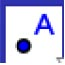
\includegraphics[scale=0.5]{images_geogebra/point.jpg}  & 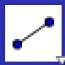
\includegraphics[scale=0.5]{images_geogebra/segment.jpg} \\ 
\hline 
Trace le point C qui est le milieu du segment [AB], et le cercle de centre
C passant par A. & 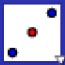
\includegraphics[scale=0.5]{images_geogebra/symetrie_centrale.jpg} & 
\includegraphics[scale=0.5]{images_geogebra/cercle.jpg}  \\ 
\hline 
Trace le point D qui est le milieu du segment [AC], puis le demi-cercle de
centre D et passant par A et C. On tracera ce demi-cercle au dessus du
segment [AC]. &  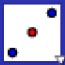
\includegraphics[scale=0.5]{images_geogebra/symetrie_centrale.jpg} &  
\includegraphics[scale=0.5]{images_geogebra/demi-cercle.jpg}\\ 
\hline 
Trace le point E qui est le milieu du segment [BC], puis le demi-cercle de
centre E et passant par B et C. On tracera ce demi-cercle en dessous du
segment [BC]. & 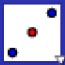
\includegraphics[scale=0.5]{images_geogebra/symetrie_centrale.jpg}  &  
\includegraphics[scale=0.5]{images_geogebra/demi-cercle.jpg} \\ 
\hline 
\end{tabular} 